\documentclass[11pt]{article}

% --------- Packages ---------
\usepackage[margin=1in]{geometry}
\usepackage{microtype}
\usepackage{booktabs}
\usepackage{tabularx}
\usepackage{enumitem}
\usepackage{hyperref}
\usepackage{xcolor}
\usepackage{tcolorbox}
\usepackage{amsmath}
\usepackage{amssymb}
\usepackage{fvextra}
\usepackage{array}
\usepackage{pgfplots}
\pgfplotsset{compat=1.18}
\usepackage{caption}
\usepackage{subcaption}

\tcbuselibrary{skins, breakable}

\definecolor{fallbackblue}{RGB}{70, 130, 180}
\definecolor{retrievalorange}{RGB}{220, 130, 40}
\definecolor{posgreen}{RGB}{34, 139, 34}
\definecolor{negred}{RGB}{205, 60, 60}

\hypersetup{
  colorlinks=true,
  linkcolor=blue,
  citecolor=blue,
  urlcolor=blue
}

% --------- Colors ---------
\definecolor{passgreen}{RGB}{40, 167, 69}
\definecolor{warnorange}{RGB}{255, 140, 0}
\definecolor{headerblue}{RGB}{70, 90, 120}
\definecolor{correctblue}{RGB}{0, 100, 200}
\definecolor{decisionbg}{RGB}{255, 248, 230}
\definecolor{decisionborder}{RGB}{255, 180, 50}

% --------- Simple macros ---------
\newcommand{\pass}{\textcolor{passgreen}{\textbf{PASS}}}
\newcommand{\fail}{\textcolor{red!70!black}{\textbf{FAIL}}}
\newcommand{\warn}{\textcolor{warnorange}{\textbf{WARN}}}

\title{MCQ Acceptance Cards: Standardized, AI-Assisted Validation of Generated Multiple-Choice Questions}
\date{\today}

\begin{document}

\maketitle

\begin{abstract}
We propose \emph{MCQ Acceptance Cards}, a lightweight and standardized framework to decide whether a generated multiple-choice question (MCQ) should be admitted into an educational question bank. Each MCQ is evaluated against a set of explicit quality dimensions. Dimensions that can be checked deterministically (e.g., JSON validity, presence of a question mark) are enforced via rules. Dimensions that require judgment (e.g., distractor plausibility, answer disclosure) are evaluated using an \emph{AI judge} (a large language model), following recent evidence that carefully elicited AI preferences can approximate human judgments at scale~\cite{bai2023rlaif}. We describe the card structure, an acceptance decision protocol, and a set of safeguards to ensure reliable and auditable use of AI judges.
\end{abstract}

\section{Motivation}
High-quality MCQs are widely used to assess learners and support adaptive practice, but authoring and validating them is time-consuming. While language models can generate MCQs, teachers and content owners face a practical bottleneck: \emph{validating} large volumes of generated items while preserving pedagogical quality and avoiding harmful artifacts (e.g., answer leakage, nonsensical distractors).

Existing evaluation pipelines often report aggregate metrics per model or per dataset. However, real deployments require \emph{item-level decisions}: should a specific generated MCQ be accepted, rejected, or revised? Moreover, many important dimensions are not purely syntactic; they require judgment, domain knowledge, and consistency. Human expert review remains the gold standard, but it does not scale.

\paragraph{Goal.}
We aim to reduce human effort by introducing a standardized artifact that (i) makes the acceptance criteria explicit and auditable, (ii) supports automatic checks when possible, and (iii) uses an AI judge \emph{only} under controlled conditions for dimensions that inherently require judgment.

\section{Problem Statement}
Given:
\begin{itemize}[leftmargin=*]
  \item Source educational material $M$ (e.g., a lesson or a LISA sheet),
  \item A generated MCQ item $q$ with four options $(a,b,c,d)$ and a designated correct option $c^\star$,
\end{itemize}
we want to decide:
\[
\texttt{Decision}(q,M) \in \{\texttt{ACCEPT},\ \texttt{REJECT},\ \texttt{REVISE}\}.
\]
The decision should be:
\begin{itemize}[leftmargin=*]
  \item \textbf{Transparent}: based on documented criteria,
  \item \textbf{Reproducible}: the same item under the same protocol yields the same decision as often as possible,
  \item \textbf{Scalable}: requires minimal expert time for large volumes,
  \item \textbf{Safe}: prevents systematic failure modes of automated judging.
\end{itemize}

\section{MCQ Acceptance Cards}
We introduce a standardized, per-item artifact: the \textbf{MCQ Acceptance Card}. It is designed to be easy to generate, easy to read, and ``hard to miss'' in the data curation workflow.

\subsection{Card Overview}
Each card contains:
\begin{enumerate}[leftmargin=*]
  \item \textbf{Metadata}: provenance and generation settings,
  \item \textbf{Deterministic Checks}: rule-based validation for non-controversial constraints,
  \item \textbf{Judgment-Based Checks}: AI-judge evaluations for subjective/semantic dimensions,
  \item \textbf{Decision Rule}: explicit acceptance policy,
  \item \textbf{Audit Trail}: minimal information to reproduce and inspect AI judgments.
\end{enumerate}

\subsection{Example Acceptance Card (Template)}

\hfuzz=3pt
\setlength{\tabcolsep}{4pt}

\begin{footnotesize}
\begin{tcolorbox}[
  enhanced,
  colback=white,
  colframe=gray!40,
  arc=4pt,
  boxrule=0.8pt,
  title={\textbf{\textcolor{white}{MCQ Acceptance Card}}},
  colbacktitle=headerblue,
  fonttitle=\bfseries\large,
  attach boxed title to top left={yshift=-2mm, xshift=4mm},
  top=6mm, left=4pt, right=4pt,
  breakable
]

% --- Header info ---
\textbf{Item ID:} MCQ-000123 \\
\textbf{Source Material:} LISA Sheet \#842 (Depression) \\
\textbf{Generator:} Llama3.1-8B (temp=0.1, top\_p=1, ctx=4096) \\
\textbf{Output Format:} JSON schema v1

\smallskip

% --- MCQ block ---
\begin{tcolorbox}[
  colback=gray!4,
  colframe=gray!30,
  arc=2pt,
  boxrule=0.5pt,
  left=6pt, right=6pt, top=4pt, bottom=4pt
]
\textbf{MCQ:}\\
Which of the following best defines a major depressive episode (MDE)?\\[4pt]
\textbf{A)} \ldots \\
\textbf{B)} \ldots \\
\textbf{C)} \ldots \\
\textbf{D)} \ldots \\[4pt]
\textcolor{correctblue}{\textbf{Correct option: C}}
\end{tcolorbox}

\smallskip

% === Section A ===
\textbf{Section A --- Deterministic Checks}
\vspace{4pt}

\begin{tabular}{@{}p{95pt}p{40pt}p{64pt}p{187pt}p{25pt}@{}}
\toprule
\textbf{Dimension} & \textbf{Result} & \textbf{Threshold} & \textbf{Notes} & \textbf{Val.} \\
\midrule
Valid JSON schema         & \pass & required   & Parsed and validated             & $\square$ \\
Question mark present     & \pass & required   & Ends with `?'                    & $\square$ \\
No leading negat.       & \pass & required   & No ``Which is \emph{not}\ldots'' & $\square$ \\
Originality (trigram)     & \pass & $\ge 0.75$ & Options not copied from stem     & $\square$ \\
Readability (FK gr.)    & \warn & $\ge 12$   & FK=11.7 (borderline)             & $\square$ \\
\bottomrule
\end{tabular}

\smallskip

% === Section B ===
\textbf{Section B --- Judgment-Based Checks}
\vspace{4pt}

\begin{tabular}{@{}p{95pt}p{40pt}p{64pt}p{187pt}p{25pt}@{}}
\toprule
\textbf{Dimension} & \textbf{Result} & \textbf{Score} & \textbf{Notes} & \textbf{Val.} \\
\midrule
Disclosure (leakage) & \pass & True/False   & Judge: not guessable by cues     & $\square$ \\
Relevance to material       & \pass & 0--1         & Judge: aligned with LISA content & $\square$ \\
Distractor plausibility     & \warn & True/False   & Judge: 3/5 average               & $\square$ \\
Difficulty appropriateness  & \pass & l/m/h        & Judge: medium                    & $\square$ \\
\bottomrule
\end{tabular}

\smallskip

% === Decision Policy ===
\begin{tcolorbox}[
  colback=decisionbg,
  colframe=decisionborder,
  arc=2pt,
  boxrule=0.8pt,
  left=6pt, right=6pt, top=4pt, bottom=4pt
]
\textbf{Decision Policy}\\
\emph{Accept if all hard constraints pass and no critical AI-judge dimension fails.}
\end{tcolorbox}

\smallskip

% === Audit Trail ===
\begin{tcolorbox}[
  colback=gray!5,
  colframe=gray!30,
  arc=2pt,
  boxrule=0.5pt,
  left=6pt, right=6pt, top=4pt, bottom=4pt
]
\textbf{Audit Trail}\\
Judge model: GPT-4o (version/date), prompt template: JUDGE\_DISTR\_V2, seed: 42,
order-swap: enabled, consistency: 2/2 stable.
\end{tcolorbox}

\smallskip

% === Accept / Refuse buttons ===
\noindent
\begin{tabularx}{\linewidth}{@{}XX@{}}
\begin{tcolorbox}[
  colback=passgreen, colframe=passgreen,
  arc=4pt, boxrule=0pt,
  halign=center, valign=center,
  height=0.8cm, left=0pt, right=0pt
]
\textcolor{white}{\Large\checkmark\ \textbf{Accept}}
\end{tcolorbox}
&
\begin{tcolorbox}[
  colback=red!75!black, colframe=red!75!black,
  arc=4pt, boxrule=0pt,
  halign=center, valign=center,
  height=0.8cm, left=0pt, right=0pt
]
\textcolor{white}{\Large$\times$\ \textbf{Refuse}}
\end{tcolorbox}
\end{tabularx}

\smallskip

% === Feedback ===
\begin{tcolorbox}[
  colback=white,
  colframe=gray!50,
  arc=2pt,
  boxrule=0.6pt,
  left=6pt, right=6pt, top=4pt, bottom=12pt
]
\textbf{Feedback:}\\[4pt]
\textcolor{gray!60}{\emph{Enter your feedback here\ldots}}
\end{tcolorbox}


\end{tcolorbox}
\end{footnotesize}

\subsection{Acceptance Policy}
We recommend making the acceptance policy explicit and configurable. A simple policy is:

\begin{itemize}[leftmargin=*]
  \item \textbf{Hard constraints} (deterministic): if any fails $\rightarrow$ \texttt{REJECT}.
  \item \textbf{Critical judgment dimensions}: if any fails $\rightarrow$ \texttt{REVISE} or \texttt{REJECT}.
  \item \textbf{Non-critical judgment dimensions}: allow small number of warnings $\rightarrow$ \texttt{REVISE}.
\end{itemize}

This separates \emph{non-negotiable} formatting and clarity constraints from \emph{quality} dimensions where revision is feasible.

\section{Syntactic dimensions}
These dimensions focus on capturing the structure of an MCQ. We provide a measure for each dimension and set empirically-verified thresholds to return a Boolean value for each of them.

{\bf Question mark.}
   We evaluate whether the question of an MCQ ends with a question mark ('?'). While not all MCQs must do so, we intentionally restrict ours to include a question mark.
   
{\bf Negation.}
    To avoid confusion, we need to filter out questions that start with a negation by verifying if a question starts with one of a pre-defined set of negations\footnote{\url{https://inspe-sciedu.gricad-pages.univ-grenoble-alpes.fr/qcm/QCM_principes.html}} and assign 1 if it does, 0 otherwise.

{\bf Originality.}
    Answers should avoid repeating the question, as this can lead to guessable answers. We propose to use trigram analysis and compare answer options to their questions. This returns 0 if more than 75\% of the trigrams (from the question) also appear in an answer option. In that case the answer is considered too similar to the question.

    A threshold of 50\% is commonly used for trigram analysis. However, since the models were consistently scoring above 50\%, we increased it to 75\%.

    Let \( T(Q) \) and \( T(A) \) be the sets of trigrams from the question and answer, respectively. The set of unique trigrams is:\\
    $T_{unique} = T(Q) \setminus T(A)$.
    
    The originality score \( O \) is then given by:
    \[
    O = \frac{| T_{unique} |}{| T(Q) |} \quad \text{(with \( O = 0 \) if \( \left| T(Q) \right| = 0 \))}
    \]
  
{\bf Readability.}
    MCQs based on educational material must be written in a formal tone and rely on discipline-specific terms. We rely on the Flesch-Kincaid grading system\footnote{\url{https://en.wikipedia.org/wiki/Flesch-Kincaid_readability_tests}} to define this measure. 
    \[
         R = 0.39\frac{total\_words}{total\_sentences}+11.8\frac{total\_syllables}{total\_words}-15.59.
    \]
    According to common practice in Education, a value greater than 12 indicates readability at the college level.

\section{Judgment-Based Dimensions and the Role of an AI Judge}
Some MCQ dimensions are not reliably captured by deterministic rules:
\begin{itemize}[leftmargin=*]
  \item \textbf{Disclosure}: does the question accidentally reveal the correct answer?
  \item \textbf{Distractor plausibility}: are distractors realistic and confusing in a pedagogically meaningful way? To compute this, we compare distractors two by two against the correct answer, asking the LLM to provide a brief justification for each plausibility score to ensure the ratings are not random. We then apply a majority vote to confirm whether the question's distractors are considered plausible.

  A known confound in LLM-based distractor evaluation is position bias: generation models systematically place the correct answer in the first position, and judge models tend to over-score the first option presented~\cite{zheng2023judging}. To neutralize this, we randomly shuffle the four options before submitting each item to the judge, updating the \texttt{correct\_option} label accordingly. This ensures that plausibility scores reflect semantic quality rather than positional priming.

  Even if the majority vote passes, we do not want the minority distractor to be trivially eliminable by students, as this would undermine item discrimination. We therefore add the constraint that every individual distractor score must be at least 2 --- ensuring no single distractor is catastrophically implausible regardless of the majority outcome.

  Finally, we apply a \textbf{rang-adaptive threshold} on the majority vote average. The LISA dataset classifies each learning objective into Rang~A (foundational knowledge) or Rang~B (applied reasoning). These ranks map directly onto Bloom's taxonomy levels~\cite{anderson2001taxonomy}: Rang~A items target recall and comprehension (levels 1--2), while Rang~B items target application and analysis (levels 3--4). For Rang~A, distractors must reach an average score of $\geq 3$; for Rang~B, the threshold is $\geq 4$. This design is grounded in \citet{haladyna2013developing}, who show that distractor quality criteria should be commensurate with the cognitive level of the item, and in \citet{gierl2017developing}, who demonstrate that nonfunctional distractors disproportionately degrade discrimination on higher-order items.

  \item \textbf{Answerability}: does the question have a single, unambiguous correct answer? We submit the question and its four options --- along with the source material as context --- to the AI judge and ask it to select the correct answer. The predicted answer is then compared to the ground-truth \texttt{correct\_option}. A mismatch signals either a flawed question stem, an incorrect ground-truth label, or distractors that are insufficiently differentiated from the correct answer.

  \item \textbf{Ambiguity}: are any distractors so semantically close to the correct answer that they could be mistaken for it? For each distractor, we compute the cosine similarity between its embedding and the embedding of the correct answer using ModernCamemBERT~\cite{labrak2023moderncamembert}. We then average these similarities across the three distractors. Following \citet{mitkov2009computer} and \citet{yeung2019difficulties}, optimal distractors occupy an intermediate similarity window --- close enough to be plausible, but distinct enough not to be interchangeable with the correct answer. The precise bounds of this window on French medical content are not yet empirically established; the metric is therefore reported as informative only, pending calibration on a representative sample.

  \item \textbf{Semantic relevance}: is the item grounded in the given material rather than the model's pretraining? To compute this, we measure the cosine similarity between the question and the source material, retaining only questions whose similarity score is greater than or equal to 0.8. Since this is a semantic comparison, a threshold closer to 0.9 would almost require the two texts to be nearly identical, making 0.8 a more reasonable and balanced choice.

  \item \textbf{Appropriate difficulty}: are options too trivial or too ambiguous? We ask the model to evaluate the difficulty of the question on a scale from 1 to 5, where 1--2 indicates low difficulty, 3 indicates medium difficulty, and 4--5 indicates high difficulty. We retain only questions rated as low or medium difficulty.
\end{itemize}

Since we are using LLMs, the key challenge is to ensure the judge is used \emph{responsibly}.

\section{Ensuring Reliable Use of AI Judges}
We adopt a set of safeguards to reduce known failure modes of LLM-as-a-judge (prompt sensitivity, position bias, inconsistency, and silent hallucinations). These safeguards turn AI judging into a more controlled and auditable component of the acceptance workflow.

\subsection{(S1) Clear, Criterion-Driven Prompts}
The judge is not asked ``is this good?'' but instead evaluates \emph{explicit criteria}. For example, for distractor quality:

\begin{tcolorbox}[colback=blue!3, colframe=blue!40, title=Judge prompt (Distractor Evaluation)]
You are an expert in educational assessment and multiple-choice question (MCQ) design.
You are given:
\begin{itemize}[leftmargin=*, itemsep=0pt, topsep=0pt]
  \item a question stem
  \item the correct answer
  \item \textbf{EXACTLY three incorrect options (distractors)}
\end{itemize}
Your task is to evaluate the quality of \textbf{EACH distractor INDIVIDUALLY}. \\
Do \textbf{NOT} give a global qualitative judgment. \\
Do \textbf{NOT} let a strong distractor compensate for weaker ones.
\medskip
\textbf{Distractor quality scale (use strictly):}
\begin{itemize}[leftmargin=*, itemsep=0pt, topsep=0pt]
  \item 1 = \textbf{POOR}: Implausible, obviously incorrect, or unrelated
  \item 2 = \textbf{BELOW AVERAGE}: Easy to eliminate, weak plausibility
  \item 3 = \textbf{AVERAGE}: Somewhat plausible but contains clear flaws
  \item 4 = \textbf{GOOD}: Plausible, reflects a common misconception
  \item 5 = \textbf{EXCELLENT}: Highly plausible, reflects a subtle misconception
\end{itemize}
For \textbf{EACH distractor}:
\begin{itemize}[leftmargin=*, itemsep=0pt, topsep=0pt]
  \item Identify the reasoning error or misconception that could lead a student to choose it.
  \item Assign a score from 1 to 5 based \textbf{ONLY} on this distractor.
  \item If no clear misconception can be identified, the score \textbf{MUST} be $\leq 2$.
  \item If the distractor is ambiguous or arguably correct, the score \textbf{MUST} be $\leq 3$.
\end{itemize}
\medskip
\textbf{Output constraints:}
\begin{itemize}[leftmargin=*, itemsep=0pt, topsep=0pt]
  \item Output \textbf{ONLY valid JSON}.
  \item Do \textbf{NOT} include explanations outside the JSON.
  \item Do \textbf{NOT} include the question, correct answer, or distractor text.
\end{itemize}
\medskip
\textbf{Output format (exactly three elements, same order as the distractors):}
\begin{Verbatim}[breaklines=true, fontsize=\small]
[
  {
    "score": <integer between 1 and 5>,
    "justif": "<brief justification of the score (1-2 sentences max)>"
  },
  {
    "score": <integer between 1 and 5>,
    "justif": "<brief justification of the score (1-2 sentences max)>"
  },
  {
    "score": <integer between 1 and 5>,
    "justif": "<brief justification of the score (1-2 sentences max)>"
  }
]
\end{Verbatim}
\end{tcolorbox}


This makes the judgment interpretable and reduces ambiguity.

\subsection{(S2) Preference/Comparison-Based Judging}
When possible, we prefer comparisons over absolute scores. For example, to reduce calibration issues, we can generate two candidate distractor sets for the same stem and ask the judge:
\begin{quote}
``Which set is more plausible and harder to eliminate for a knowledgeable student, and why?''
\end{quote}
This produces a \emph{preference} signal (A vs B), which is often more stable than raw numeric scoring.

\subsection{(S3) Position-Bias Mitigation via Random Shuffling}
LLMs exhibit position bias: generation models tend to place the correct answer in the first position, and judge models tend to over-score the first option presented~\cite{zheng2023judging}. We mitigate this by randomly shuffling the four options before each judge call and updating the \texttt{correct\_option} label accordingly, so that the judge never systematically evaluates the correct answer or any distractor in a fixed position.

\subsection{(S4) Self-Consistency and Majority Voting}
We can query the judge $k$ times with controlled randomness (or multiple judges) and aggregate:
\begin{itemize}[leftmargin=*]
  \item \textbf{Discrete outputs}: majority vote
  \item \textbf{Scores}: median and dispersion (e.g., IQR)
\end{itemize}
High dispersion triggers \warn\ and optionally human review.

\subsection{(S5) Confidence Filtering and ``Abstain'' Option}
The judge is instructed to abstain when uncertain (e.g., ``INSUFFICIENT\_INFO''). Items with abstentions are not automatically accepted. This avoids false confidence.

\subsection{(S6) Grounding Requirements}
For dimensions that depend on source material, the judge must cite short evidence snippets from $M$ (or point to section titles). If it cannot ground the answer, it should abstain.

\subsection{(S7) Audit Trail and Reproducibility}
Each card stores the minimal audit info:
\begin{itemize}[leftmargin=*]
  \item judge model name/version,
  \item prompt template ID and parameters,
  \item decoding settings,
  \item number of trials and aggregation method,
  \item whether order swaps were used and whether judgments were stable.
\end{itemize}
This supports later debugging, re-running, or comparing judges.

\section{Embedding Model for Semantic Metrics}
The Relevance and Ambiguity metrics both rely on dense text representations. We use \texttt{almanach/moderncamembert-base} (ModernCamemBERT)~\cite{labrak2023moderncamembert}, a French encoder pre-trained on large-scale French corpora. We deliberately chose a French-language encoder over multilingual or English-only alternatives (e.g.\ \texttt{BAAI/bge-base-en-v1.5}) to preserve the semantic structure of French medical terminology, which is systematically degraded by English-trained models.

\section{Reliability of the AI Judge}

\textit{Note: reliability experiments are not yet conducted. The methodology below is defined and the scripts are implemented; results will be added once runs are complete.}

\subsection{Intra-rater Reliability}
To assess the stability of the LLM judge, we submit the same MCQ twice to the judge under identical conditions and measure the variance in distractor plausibility scores across the two runs. We report the mean absolute difference and standard deviation per distractor, as well as the PASS/FAIL agreement rate. A mean absolute difference below 0.5 points is considered acceptable, following the convention for human rater consistency in educational measurement~\cite{stemler2004comparison}. High variance would indicate that scores are driven by stochastic sampling rather than genuine quality assessment.

\subsection{Inter-rater Reliability}
To validate the AI judge against human judgment, a subset of 30--50 MCQs is annotated manually by a domain expert using the same 1--5 plausibility scale. We compute linear Cohen's $\kappa$ between the AI scores and the human annotations, targeting $\kappa \geq 0.6$, corresponding to substantial agreement~\cite{landis1977measurement}. This step confirms that the AI judge captures the same construct as an expert medical examiner, rather than a proxy correlated with surface-level lexical features.

\section{How Cards Integrate into a Curation Pipeline}
Cards can be generated automatically and used as a gating mechanism:
\begin{enumerate}[leftmargin=*]
  \item Generate candidate MCQs from material $M$,
  \item Build Acceptance Cards for each MCQ:
  \begin{itemize}[leftmargin=*]
    \item Run deterministic checks,
    \item Run AI-judge checks with safeguards,
    \item Apply acceptance policy,
  \end{itemize}
  \item Store:
  \begin{itemize}[leftmargin=*]
    \item accepted items into the MCQ bank,
    \item rejected items (with reasons) into an error log,
    \item revise items into a ``repair'' queue (potentially handled by a rewriting model).
  \end{itemize}
\end{enumerate}

\section{Experimental Evaluation}
\label{sec:eval}

We evaluated 11 language models on a corpus of LISA sheets using two prompt strategies: a \emph{fallback} prompt (generic, no retrieval) and a \emph{retrieval} prompt that injects the source content at query time. Each generated MCQ was scored by the acceptance pipeline, and the proportion of items reaching \emph{good quality} (all judgment-based dimensions passing) is reported below.

Figure~\ref{fig:grouped-bar} compares the two prompts across all models. Figures~\ref{fig:delta} and~\ref{fig:kto} break down the delta per model and zoom in on the effect of KTO fine-tuning.

%% ---- Figure 1: grouped bar chart ----
\begin{figure}[htbp]
\centering
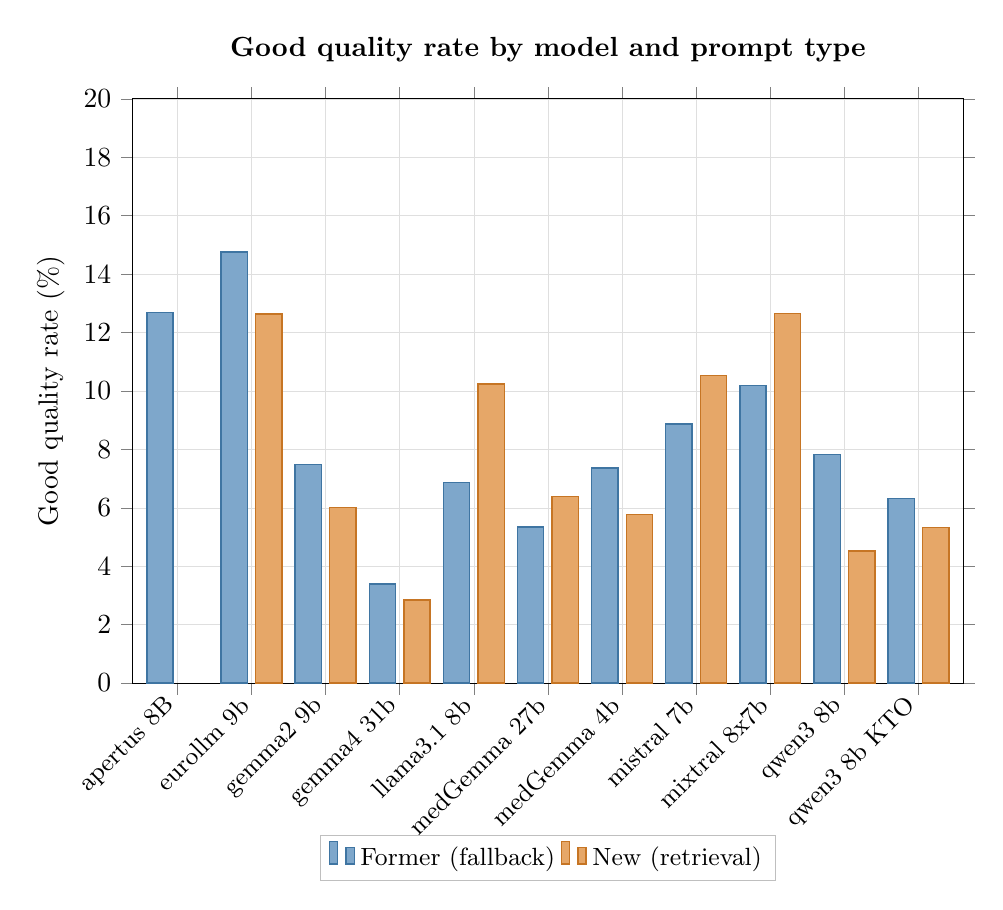
\begin{tikzpicture}
\begin{axis}[
    ybar=3pt,
    bar width=9.5pt,
    width=\textwidth,
    height=9cm,
    legend style={
        at={(0.5,-0.26)},
        anchor=north,
        legend columns=2,
        font=\small,
        draw=gray!50,
    },
    ylabel={Good quality rate (\%)},
    xtick={0,1,2,3,4,5,6,7,8,9,10},
    xticklabels={
        apertus 8B,
        eurollm 9b,
        gemma2 9b,
        gemma4 31b,
        llama3.1 8b,
        medGemma 27b,
        medGemma 4b,
        mistral 7b,
        mixtral 8x7b,
        qwen3 8b,
        qwen3 8b KTO
    },
    x tick label style={rotate=45, anchor=east, font=\small},
    ymin=0, ymax=20,
    enlarge x limits=0.06,
    grid=major,
    grid style={line width=.2pt, draw=gray!25},
    tick align=outside,
    title={Good quality rate by model and prompt type},
    title style={font=\normalsize\bfseries, yshift=4pt},
]
\addplot[fill=fallbackblue!70, draw=fallbackblue!90!black, line width=0.5pt] coordinates {
    (0, 12.68) (1, 14.76) (2,  7.48) (3,  3.39) (4,  6.86)
    (5,  5.35) (6,  7.37) (7,  8.87) (8, 10.19) (9,  7.82) (10, 6.32)
};
\addplot[fill=retrievalorange!70, draw=retrievalorange!90!black, line width=0.5pt] coordinates {
    (1, 12.64) (2,  6.02) (3,  2.84) (4, 10.24) (5,  6.38)
    (6,  5.77) (7, 10.54) (8, 12.65) (9,  4.52) (10, 5.33)
};
\legend{Former (fallback), New (retrieval)}
\end{axis}
\end{tikzpicture}
\caption{Good quality rate per model and prompt type.
\textit{apertus}~8B has no retrieval-prompt data ($n=1\,096$ evaluations).}
\label{fig:grouped-bar}
\end{figure}

%% ---- Figure 2: delta + KTO focus ----
\begin{figure}[htbp]
\centering
\begin{subfigure}[b]{0.60\textwidth}
\centering
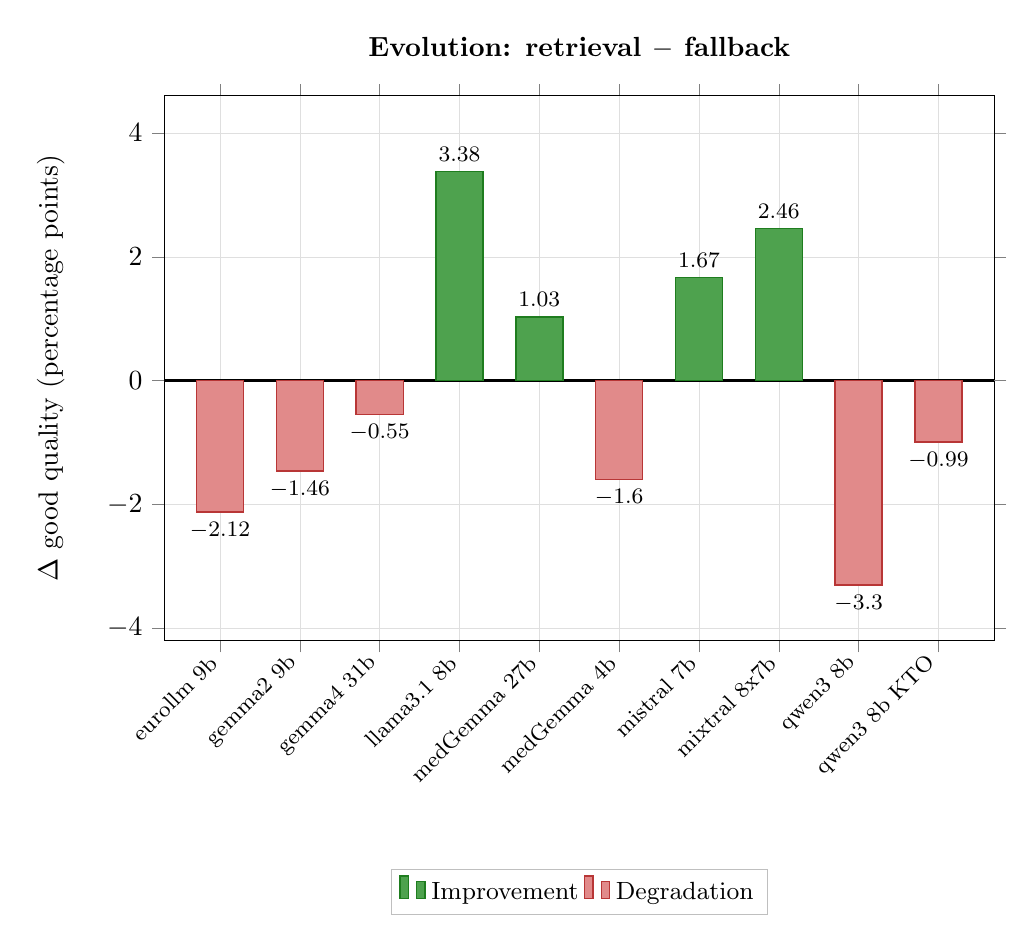
\begin{tikzpicture}
\begin{axis}[
    ybar,
    bar width=17pt,
    width=\textwidth,
    height=8.5cm,
    ylabel={$\Delta$ good quality (percentage points)},
    xtick={1,2,3,4,5,6,7,8,9,10},
    xticklabels={
        eurollm 9b,
        gemma2 9b,
        gemma4 31b,
        llama3.1 8b,
        medGemma 27b,
        medGemma 4b,
        mistral 7b,
        mixtral 8x7b,
        qwen3 8b,
        qwen3 8b KTO
    },
    x tick label style={rotate=45, anchor=east, font=\footnotesize},
    ymin=-4.2, ymax=4.6,
    xmin=0.3, xmax=10.7,
    grid=major,
    grid style={line width=.2pt, draw=gray!25},
    extra y ticks={0},
    extra y tick style={
        grid=major,
        grid style={black, line width=1.2pt},
        tick label style={draw=none},
    },
    extra y tick labels={},
    nodes near coords,
    nodes near coords align={vertical},
    every node near coord/.append style={font=\footnotesize},
    tick align=outside,
    legend style={
        at={(0.5,-0.42)},
        anchor=north,
        legend columns=2,
        font=\small,
        draw=gray!50,
    },
    title={Evolution: retrieval $-$ fallback},
    title style={font=\normalsize\bfseries, yshift=4pt},
]
\addplot[fill=posgreen!80, draw=posgreen!90!black, line width=0.5pt, bar shift=0pt] coordinates {
    (4, 3.38) (5, 1.03) (7, 1.67) (8, 2.46)
};
\addlegendentry{Improvement}
\addplot[fill=negred!60, draw=negred!90!black, line width=0.5pt, bar shift=0pt] coordinates {
    (1, -2.12) (2, -1.46) (3, -0.55) (6, -1.60) (9, -3.30) (10, -0.99)
};
\addlegendentry{Degradation}
\end{axis}
\end{tikzpicture}
\caption{Delta in percentage points (retrieval $-$ fallback).\\
\textcolor{posgreen}{\textbf{Green}}: improvement;
\textcolor{negred}{\textbf{Red}}: degradation.}
\label{fig:delta}
\end{subfigure}
\hfill
\begin{subfigure}[b]{0.37\textwidth}
\centering
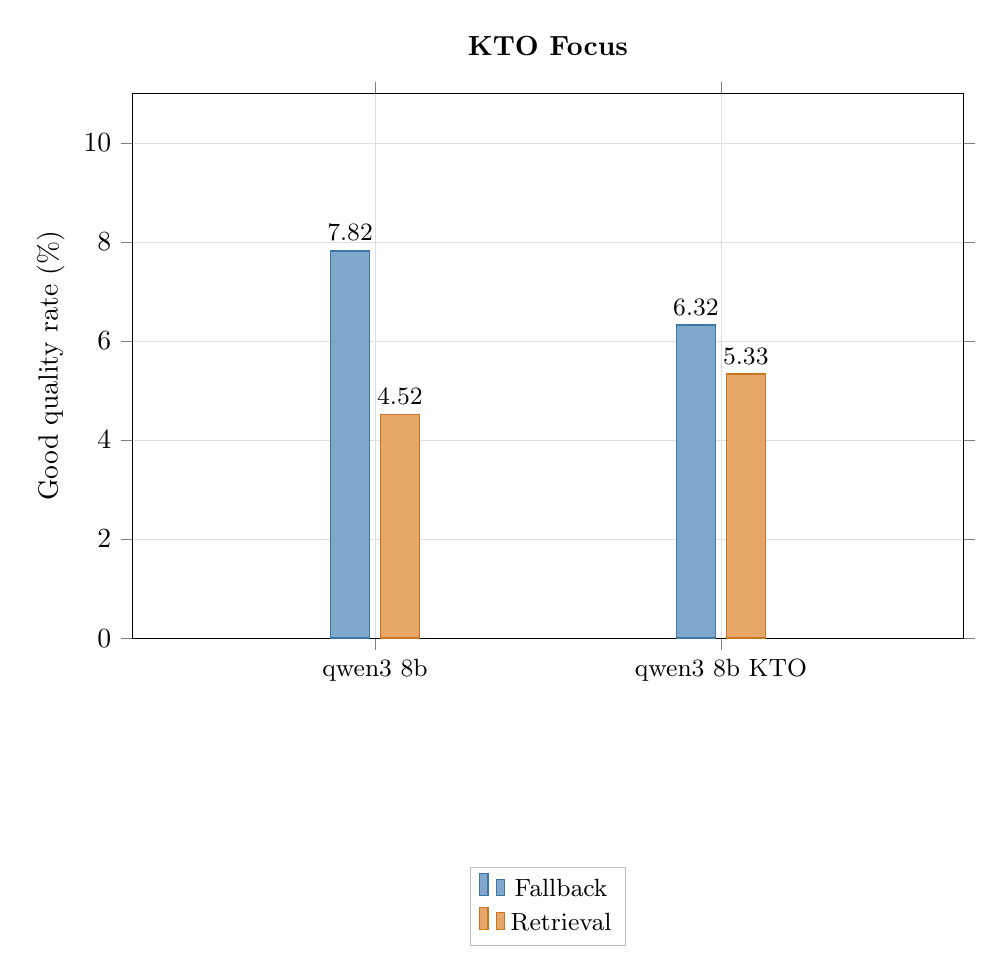
\begin{tikzpicture}
\begin{axis}[
    ybar=4pt,
    bar width=14pt,
    width=\textwidth,
    height=8.5cm,
    legend style={
        at={(0.5,-0.42)},
        anchor=north,
        legend columns=1,
        font=\small,
        draw=gray!50,
    },
    ylabel={Good quality rate (\%)},
    xtick={0,1},
    xticklabels={qwen3 8b, qwen3 8b KTO},
    x tick label style={font=\small},
    ymin=0, ymax=11,
    xmin=-0.7, xmax=1.7,
    nodes near coords,
    nodes near coords align={vertical},
    every node near coord/.append style={font=\small},
    grid=major,
    grid style={line width=.2pt, draw=gray!25},
    tick align=outside,
    title={KTO Focus},
    title style={font=\normalsize\bfseries, yshift=4pt},
]
\addplot[fill=fallbackblue!70, draw=fallbackblue!90!black, line width=0.5pt] coordinates {
    (0, 7.82) (1, 6.32)
};
\addplot[fill=retrievalorange!70, draw=retrievalorange!90!black, line width=0.5pt] coordinates {
    (0, 4.52) (1, 5.33)
};
\legend{Fallback, Retrieval}
\end{axis}
\end{tikzpicture}
\caption{Base model vs.\ KTO fine-tuned variant by prompt type.}
\label{fig:kto}
\end{subfigure}
\caption{Left: change in good quality rate (retrieval~$-$~fallback) per model
(excluding \textit{apertus}~8B, not evaluated under retrieval).
Right: focus on \textit{qwen3}~8b and its KTO variant.}
\label{fig:delta-kto}
\end{figure}

\section{Discussion and Expected Benefits}
\paragraph{Reduced human effort.}
Teachers no longer need to inspect every generated item. Instead, they can:
\begin{itemize}[leftmargin=*]
  \item review only \texttt{REVISE} items,
  \item spot-check a small sample of \texttt{ACCEPT} items,
  \item adjust thresholds depending on pedagogical goals.
\end{itemize}

\paragraph{Transparency and governance.}
Cards provide a structured record of why items were accepted or rejected, making it easier to:
\begin{itemize}[leftmargin=*]
  \item communicate quality criteria,
  \item reproduce curation decisions,
  \item audit failures and improve prompts/thresholds.
\end{itemize}

\paragraph{Future extensions.}
Cards can naturally support:
\begin{itemize}[leftmargin=*]
  \item targeted fine-tuning (e.g., improve distractor quality),
  \item teacher personalization (e.g., stricter readability, different difficulty),
  \item tracking drift across model versions.
\end{itemize}

\section{Conclusion}
MCQ Acceptance Cards turn multi-dimensional evaluation into an item-level, standardized, and auditable acceptance protocol. By combining deterministic checks with carefully controlled AI judging, the framework enables scalable curation of MCQs while preserving transparency and leaving room for human oversight where needed.

\bibliographystyle{plain}
\bibliography{biblio}

\end{document}
